\chapter{INSTALLATION}
\section{Obtain}

The {\iqist} is an open source free software package. We release it under the General Public Licence 3.0 (GPL). The readers who are interested in it can write a letter to the authors to request an electronic copy of the newest version of {\iqist}:
 
\noindent\colorbox{pink}{\parbox[r]{\linewidth}{\quad email: huangli712@gmail.com,}}
or they can download it directly from the public code repository:

\noindent\colorbox{pink}{\parbox[r]{\linewidth}{\quad http://bitbucket.org/huangli712/iqist.}}

\section{Uncompress}

The downloaded {\iqist} software package is likely a compressed file with zip or tar.gz suffix. The users should uncompress it at first. For examples:

\noindent\colorbox{pink}{\parbox[r]{\linewidth}{\quad \$ tar xvfz iqist.tar.gz.}}

\section{Direcrory structures}

\begin{figure}
\centering
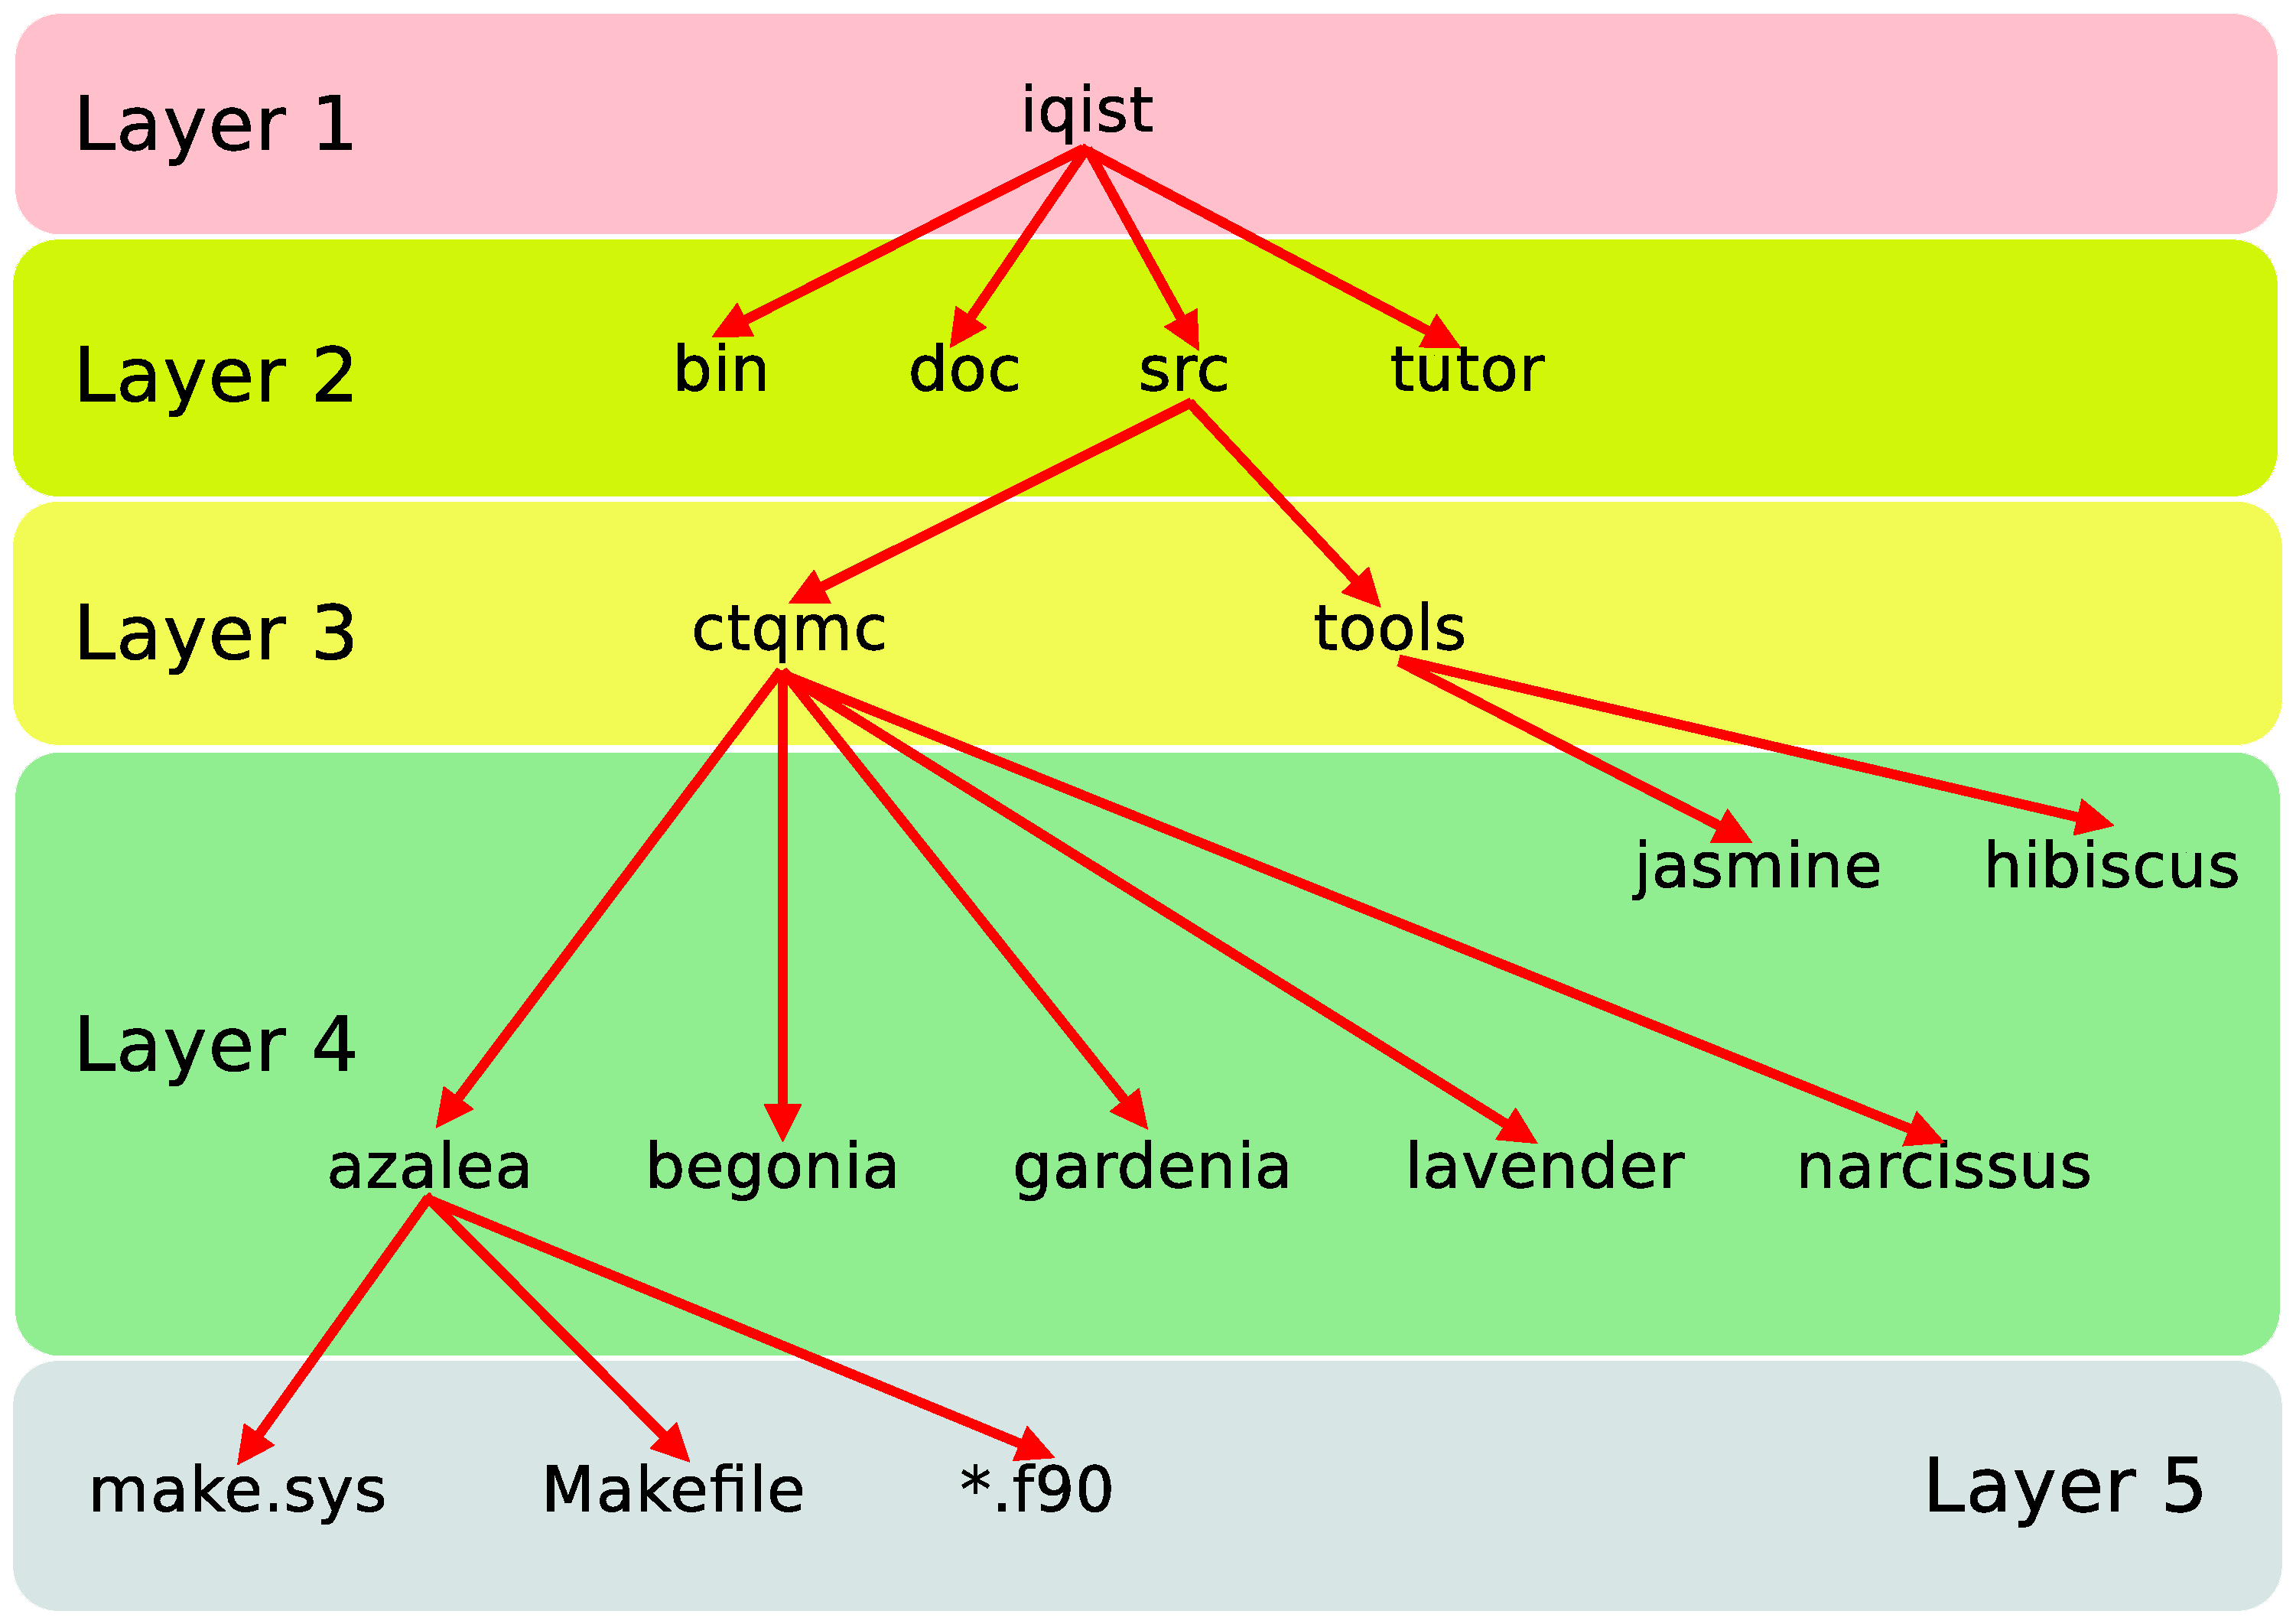
\includegraphics[scale=0.28]{figure/dir.eps}
\caption{The directory structure of {\iqist} software package.\label{fig:dir}}
\end{figure}

The directory structure of the {\iqist} software package is shown in Fig.~\ref{fig:dir}.

\section{Compiling environment}

In order to compile and install {\iqist} correctly, you should ensure the following softwares are correctly installed and configured in your OS.
\begin{itemize}
\item Intel Fortran compiler
\item MPICH2 or OpenMPI
\item BLAS
\item LAPACK
\item Python 2.X
\item scipy, numpy, and f2py
\end{itemize}
The components in {\iqist} can be successfully compiled using a recent Intel Fortran compiler. Most of the MPI implementations, such as MPICH, MVAPICH, OpenMPI and Intel MPI are compatible with {\iqist}. As for the BLAS implementation, we strongly recommend OpenBLAS. For the LAPACK, the Intel Math Kernel Library is a good candidate. Of course, it is also possible to use the linear algebra library provided by the operating system, for example, the vecLib Framework in the Mac OS X. Some post-processing scripts contained in the {\hibiscus} component are developed using the Python language. In order to execute these scripts or use the Python language binding for {\iqist}, the users should install Python 2.x. Furthermore, the numpy, scipy, and f2py packages are also necessary.

\section{Compiling system}

And then go to the iqist/src/build directory, edit the make.sys file to configure the compiling environment. The users must setup the Fortran compiler, MPI compiler, BLAS and LAPACK libraries manually. Once the compiling environment is configured, run the make command in the top-level directory of {\iqist}. After a few minutes (depending on the performance of compiling platform), the {\iqist} is ready for use. Note that all of the executable programs will be copied into the iqist/bin directory automatically. Please add this directory into the system environment variable PATH.

\section{Build quantum impurity solvers}
\section{Build auxiliary tools}
\section{Build documents}
\section{Build library}
\section{Build application programming interfaces}
